

\tikzset{every picture/.style={line width=0.75pt}} %set default line width to 0.75pt        

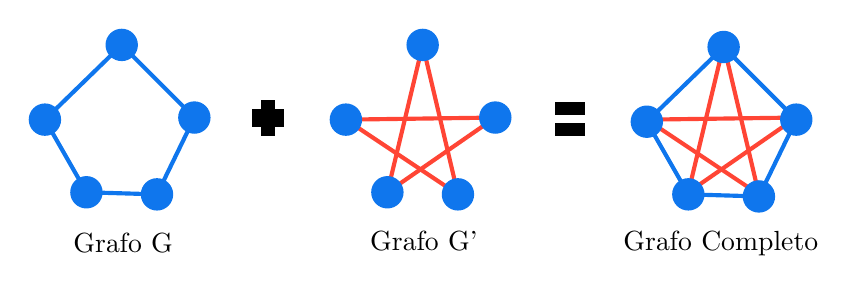
\begin{tikzpicture}[x=0.75pt,y=0.75pt,yscale=-1,xscale=1]
%uncomment if require: \path (0,146); %set diagram left start at 0, and has height of 146

%Straight Lines [id:da6286716115891509] 
\draw [color={rgb, 255:red, 255; green, 69; blue, 53 }  ,draw opacity=1 ][line width=1.5]    (388.81,99.81) -- (371.81,27.81) ;
%Straight Lines [id:da8615097224096446] 
\draw [color={rgb, 255:red, 255; green, 69; blue, 53 }  ,draw opacity=1 ][line width=1.5]    (406.81,62.81) -- (334.81,63.81) ;
%Straight Lines [id:da6874816210575747] 
\draw [color={rgb, 255:red, 255; green, 69; blue, 53 }  ,draw opacity=1 ][line width=1.5]    (388.81,99.81) -- (334.81,63.81) ;
%Straight Lines [id:da7467287538393712] 
\draw [color={rgb, 255:red, 255; green, 69; blue, 53 }  ,draw opacity=1 ][line width=1.5]    (354.81,98.81) -- (406.81,62.81) ;
%Straight Lines [id:da22709598157536104] 
\draw [color={rgb, 255:red, 255; green, 69; blue, 53 }  ,draw opacity=1 ][line width=1.5]    (371.81,27.81) -- (354.81,98.81) ;
%Straight Lines [id:da8128576904560505] 
\draw [color={rgb, 255:red, 255; green, 69; blue, 53 }  ,draw opacity=1 ][line width=1.5]    (243.81,99.81) -- (226.81,27.81) ;
%Straight Lines [id:da46056102558920564] 
\draw [color={rgb, 255:red, 255; green, 69; blue, 53 }  ,draw opacity=1 ][line width=1.5]    (261.81,62.81) -- (189.81,63.81) ;
%Straight Lines [id:da5780673278719084] 
\draw [color={rgb, 255:red, 255; green, 69; blue, 53 }  ,draw opacity=1 ][line width=1.5]    (243.81,99.81) -- (189.81,63.81) ;
%Straight Lines [id:da10083150854017786] 
\draw [color={rgb, 255:red, 255; green, 69; blue, 53 }  ,draw opacity=1 ][line width=1.5]    (209.81,98.81) -- (261.81,62.81) ;
%Straight Lines [id:da39379403255252776] 
\draw [color={rgb, 255:red, 255; green, 69; blue, 53 }  ,draw opacity=1 ][line width=1.5]    (226.81,27.81) -- (209.81,98.81) ;
%Shape: Circle [id:dp17206767364522735] 
\draw  [draw opacity=0][fill={rgb, 255:red, 15; green, 118; blue, 237 }  ,fill opacity=1 ] (74,27.81) .. controls (74,23.49) and (77.49,20) .. (81.81,20) .. controls (86.12,20) and (89.61,23.49) .. (89.61,27.81) .. controls (89.61,32.12) and (86.12,35.61) .. (81.81,35.61) .. controls (77.49,35.61) and (74,32.12) .. (74,27.81) -- cycle ;
%Shape: Circle [id:dp8817745518555591] 
\draw  [draw opacity=0][fill={rgb, 255:red, 15; green, 118; blue, 237 }  ,fill opacity=1 ] (91,99.81) .. controls (91,95.49) and (94.49,92) .. (98.81,92) .. controls (103.12,92) and (106.61,95.49) .. (106.61,99.81) .. controls (106.61,104.12) and (103.12,107.61) .. (98.81,107.61) .. controls (94.49,107.61) and (91,104.12) .. (91,99.81) -- cycle ;
%Shape: Circle [id:dp983446861828384] 
\draw  [draw opacity=0][fill={rgb, 255:red, 15; green, 118; blue, 237 }  ,fill opacity=1 ] (109,62.81) .. controls (109,58.49) and (112.49,55) .. (116.81,55) .. controls (121.12,55) and (124.61,58.49) .. (124.61,62.81) .. controls (124.61,67.12) and (121.12,70.61) .. (116.81,70.61) .. controls (112.49,70.61) and (109,67.12) .. (109,62.81) -- cycle ;
%Shape: Circle [id:dp3733314601313251] 
\draw  [draw opacity=0][fill={rgb, 255:red, 15; green, 118; blue, 237 }  ,fill opacity=1 ] (57,98.81) .. controls (57,94.49) and (60.49,91) .. (64.81,91) .. controls (69.12,91) and (72.61,94.49) .. (72.61,98.81) .. controls (72.61,103.12) and (69.12,106.61) .. (64.81,106.61) .. controls (60.49,106.61) and (57,103.12) .. (57,98.81) -- cycle ;
%Shape: Circle [id:dp31508397542449407] 
\draw  [draw opacity=0][fill={rgb, 255:red, 15; green, 118; blue, 237 }  ,fill opacity=1 ] (37,63.81) .. controls (37,59.49) and (40.49,56) .. (44.81,56) .. controls (49.12,56) and (52.61,59.49) .. (52.61,63.81) .. controls (52.61,68.12) and (49.12,71.61) .. (44.81,71.61) .. controls (40.49,71.61) and (37,68.12) .. (37,63.81) -- cycle ;
%Straight Lines [id:da4019504678384127] 
\draw [color={rgb, 255:red, 15; green, 118; blue, 237 }  ,draw opacity=1 ][line width=1.5]    (44.81,63.81) -- (81.81,27.81) ;
%Straight Lines [id:da33751766037536557] 
\draw [color={rgb, 255:red, 15; green, 118; blue, 237 }  ,draw opacity=1 ][line width=1.5]    (116.81,62.81) -- (81.81,27.81) ;
%Straight Lines [id:da36837524239373765] 
\draw [color={rgb, 255:red, 15; green, 118; blue, 237 }  ,draw opacity=1 ][line width=1.5]    (64.81,98.81) -- (44.81,63.81) ;
%Straight Lines [id:da5684634535440216] 
\draw [color={rgb, 255:red, 15; green, 118; blue, 237 }  ,draw opacity=1 ][line width=1.5]    (98.81,99.81) -- (116.81,62.81) ;
%Straight Lines [id:da7336404196898463] 
\draw [color={rgb, 255:red, 15; green, 118; blue, 237 }  ,draw opacity=1 ][line width=1.5]    (64.81,98.81) -- (98.81,99.81) ;
%Shape: Circle [id:dp2133071752077793] 
\draw  [draw opacity=0][fill={rgb, 255:red, 15; green, 118; blue, 237 }  ,fill opacity=1 ] (219,27.81) .. controls (219,23.49) and (222.49,20) .. (226.81,20) .. controls (231.12,20) and (234.61,23.49) .. (234.61,27.81) .. controls (234.61,32.12) and (231.12,35.61) .. (226.81,35.61) .. controls (222.49,35.61) and (219,32.12) .. (219,27.81) -- cycle ;
%Shape: Circle [id:dp7970171128213852] 
\draw  [draw opacity=0][fill={rgb, 255:red, 15; green, 118; blue, 237 }  ,fill opacity=1 ] (236,99.81) .. controls (236,95.49) and (239.49,92) .. (243.81,92) .. controls (248.12,92) and (251.61,95.49) .. (251.61,99.81) .. controls (251.61,104.12) and (248.12,107.61) .. (243.81,107.61) .. controls (239.49,107.61) and (236,104.12) .. (236,99.81) -- cycle ;
%Shape: Circle [id:dp8772839428999042] 
\draw  [draw opacity=0][fill={rgb, 255:red, 15; green, 118; blue, 237 }  ,fill opacity=1 ] (254,62.81) .. controls (254,58.49) and (257.49,55) .. (261.81,55) .. controls (266.12,55) and (269.61,58.49) .. (269.61,62.81) .. controls (269.61,67.12) and (266.12,70.61) .. (261.81,70.61) .. controls (257.49,70.61) and (254,67.12) .. (254,62.81) -- cycle ;
%Shape: Circle [id:dp08146825073335462] 
\draw  [draw opacity=0][fill={rgb, 255:red, 15; green, 118; blue, 237 }  ,fill opacity=1 ] (202,98.81) .. controls (202,94.49) and (205.49,91) .. (209.81,91) .. controls (214.12,91) and (217.61,94.49) .. (217.61,98.81) .. controls (217.61,103.12) and (214.12,106.61) .. (209.81,106.61) .. controls (205.49,106.61) and (202,103.12) .. (202,98.81) -- cycle ;
%Shape: Circle [id:dp2604299443287845] 
\draw  [draw opacity=0][fill={rgb, 255:red, 15; green, 118; blue, 237 }  ,fill opacity=1 ] (182,63.81) .. controls (182,59.49) and (185.49,56) .. (189.81,56) .. controls (194.12,56) and (197.61,59.49) .. (197.61,63.81) .. controls (197.61,68.12) and (194.12,71.61) .. (189.81,71.61) .. controls (185.49,71.61) and (182,68.12) .. (182,63.81) -- cycle ;
%Shape: Circle [id:dp02208476926602243] 
\draw  [draw opacity=0][fill={rgb, 255:red, 15; green, 118; blue, 237 }  ,fill opacity=1 ] (364,28.81) .. controls (364,24.49) and (367.49,21) .. (371.81,21) .. controls (376.12,21) and (379.61,24.49) .. (379.61,28.81) .. controls (379.61,33.12) and (376.12,36.61) .. (371.81,36.61) .. controls (367.49,36.61) and (364,33.12) .. (364,28.81) -- cycle ;
%Shape: Circle [id:dp14745587301806817] 
\draw  [draw opacity=0][fill={rgb, 255:red, 15; green, 118; blue, 237 }  ,fill opacity=1 ] (381,100.81) .. controls (381,96.49) and (384.49,93) .. (388.81,93) .. controls (393.12,93) and (396.61,96.49) .. (396.61,100.81) .. controls (396.61,105.12) and (393.12,108.61) .. (388.81,108.61) .. controls (384.49,108.61) and (381,105.12) .. (381,100.81) -- cycle ;
%Shape: Circle [id:dp03821434537628687] 
\draw  [draw opacity=0][fill={rgb, 255:red, 15; green, 118; blue, 237 }  ,fill opacity=1 ] (399,63.81) .. controls (399,59.49) and (402.49,56) .. (406.81,56) .. controls (411.12,56) and (414.61,59.49) .. (414.61,63.81) .. controls (414.61,68.12) and (411.12,71.61) .. (406.81,71.61) .. controls (402.49,71.61) and (399,68.12) .. (399,63.81) -- cycle ;
%Shape: Circle [id:dp14052332172014892] 
\draw  [draw opacity=0][fill={rgb, 255:red, 15; green, 118; blue, 237 }  ,fill opacity=1 ] (347,99.81) .. controls (347,95.49) and (350.49,92) .. (354.81,92) .. controls (359.12,92) and (362.61,95.49) .. (362.61,99.81) .. controls (362.61,104.12) and (359.12,107.61) .. (354.81,107.61) .. controls (350.49,107.61) and (347,104.12) .. (347,99.81) -- cycle ;
%Shape: Circle [id:dp08749177881137715] 
\draw  [draw opacity=0][fill={rgb, 255:red, 15; green, 118; blue, 237 }  ,fill opacity=1 ] (327,64.81) .. controls (327,60.49) and (330.49,57) .. (334.81,57) .. controls (339.12,57) and (342.61,60.49) .. (342.61,64.81) .. controls (342.61,69.12) and (339.12,72.61) .. (334.81,72.61) .. controls (330.49,72.61) and (327,69.12) .. (327,64.81) -- cycle ;
%Straight Lines [id:da0162842505226648] 
\draw [color={rgb, 255:red, 15; green, 118; blue, 237 }  ,draw opacity=1 ][line width=1.5]    (334.81,64.81) -- (371.81,28.81) ;
%Straight Lines [id:da5332427745678958] 
\draw [color={rgb, 255:red, 15; green, 118; blue, 237 }  ,draw opacity=1 ][line width=1.5]    (406.81,63.81) -- (371.81,28.81) ;
%Straight Lines [id:da906855391597275] 
\draw [color={rgb, 255:red, 15; green, 118; blue, 237 }  ,draw opacity=1 ][line width=1.5]    (354.81,99.81) -- (334.81,64.81) ;
%Straight Lines [id:da09115093571142174] 
\draw [color={rgb, 255:red, 15; green, 118; blue, 237 }  ,draw opacity=1 ][line width=1.5]    (388.81,100.81) -- (406.81,63.81) ;
%Straight Lines [id:da591316390817122] 
\draw [color={rgb, 255:red, 15; green, 118; blue, 237 }  ,draw opacity=1 ][line width=1.5]    (354.81,99.81) -- (388.81,100.81) ;
%Shape: Cross [id:dp6301285378327248] 
\draw  [fill={rgb, 255:red, 0; green, 0; blue, 0 }  ,fill opacity=1 ] (149.38,55.01) -- (155.22,55.01) -- (155.22,59.39) -- (159.61,59.39) -- (159.61,66.62) -- (155.22,66.62) -- (155.22,71) -- (149.38,71) -- (149.38,66.62) -- (145,66.62) -- (145,59.39) -- (149.38,59.39) -- cycle ;
%Shape: Rectangle [id:dp5532971331016707] 
\draw  [fill={rgb, 255:red, 0; green, 0; blue, 0 }  ,fill opacity=1 ] (291,56) -- (304.61,56) -- (304.61,61.01) -- (291,61.01) -- cycle ;
%Shape: Rectangle [id:dp852512220039451] 
\draw  [fill={rgb, 255:red, 0; green, 0; blue, 0 }  ,fill opacity=1 ] (291,66) -- (304.61,66) -- (304.61,71.01) -- (291,71.01) -- cycle ;

% Text Node
\draw (57,117) node [anchor=north west][inner sep=0.75pt]   [align=left] {Grafo G};
% Text Node
\draw (200,115.97) node [anchor=north west][inner sep=0.75pt]   [align=left] {Grafo G'};
% Text Node
\draw (322,115.97) node [anchor=north west][inner sep=0.75pt]   [align=left] {Grafo Completo};


\end{tikzpicture}